\documentclass[a4paper,12pt]{article}

\usepackage{cmap}					
\usepackage[T2A]{fontenc}			
\usepackage[utf8]{inputenc}			
\usepackage[english,russian]{babel}	

\usepackage{amsmath,amsfonts,amssymb,amsthm,mathtools} 
\usepackage{wasysym}


\usepackage{graphicx}
\usepackage[cache=false]{minted}

\usepackage{indentfirst}
\usepackage{amssymb}


\usepackage{listings} 
\usepackage{fancyvrb}
%\DefineShortVerb{\|}

\usepackage{color}
\usepackage{caption}
\DeclareCaptionFont{white}{\color{black}}
\DeclareCaptionFormat{listing}{\colorbox{white}{\parbox{\textwidth}{#1#2#3}}}
\captionsetup[lstlisting]{format=listing,labelfont=white,textfont=white}


\usepackage{listings}

\usepackage{geometry}
\geometry{left=2cm}
\geometry{right=1.5cm}
\geometry{top=1cm}
\geometry{bottom=2cm}
\setlength{\parindent}{5ex}
\setlength{\parskip}{0.5em}

\begin{document} % Конец преамбулы, начало текста.

\lstset{ %
language=C++,                 % выбор языка для подсветки (здесь это С)
basicstyle=\small\sffamily, % размер и начертание шрифта для подсветки кода
numbers=left,               % где поставить нумерацию строк (слева\справа)
numberstyle=\tiny,           % размер шрифта для номеров строк
stepnumber=1,                   % размер шага между двумя номерами строк
numbersep=5pt,                % как далеко отстоят номера строк от подсвечиваемого кода
backgroundcolor=\color{white}, % цвет фона подсветки - используем \usepackage{color}
showspaces=false,            % показывать или нет пробелы специальными отступами
showstringspaces=false,      % показывать или нет пробелы в строках
showtabs=false,             % показывать или нет табуляцию в строках
frame=single,              % рисовать рамку вокруг кода
tabsize=2,                 % размер табуляции по умолчанию равен 2 пробелам
captionpos=t,              % позиция заголовка вверху [t] или внизу [b] 
breaklines=true,           % автоматически переносить строки (да\нет)
breakatwhitespace=false, % переносить строки только если есть пробел
escapeinside={\%*}{*)}   % если нужно добавить комментарии в коде
}


\large
\begin{center}
Федеральное государственное бюджетное образовательное учреждение высшего образования «Московский государственный технический университет имени Н. Э. Баумана (национальный исследовательский университет»)
\end{center}

\vspace*{30mm} 

\LARGE
\begin{center}
Курс: <<Анализ алгоритмов>>

Лабораторная работа №3
\end{center}

\vspace*{30mm} 

\huge
\begin{center}
Тема работы:\\
<<Сортировка массивов>>
\end{center}
\vspace*{30mm} 

\large
\begin{flushright}
Студент: Волков Е. А. \\
Преподаватели: Волкова Л. Л. \\
				Строганов Ю. В. \\
Группа: ИУ7-55Б
\end{flushright}

\vspace*{40mm}
\begin{center}
2019    
\end{center}
\thispagestyle{empty}
\pagebreak


\tableofcontents
\pagebreak


\section*{Введение}
\addcontentsline{toc}{section}{Введение}

Цель лабораторной работы: изучение метода динамического программирования на материале алгоритмов сортировок массивов, а именно: на сортировке пузырьком, сортировке слиянием и быстрой сортировке.

Задачи работы:

	
\begin{enumerate} 
	
	\item[1)] изучение алгоритмов сортировок;
	\item[2)] применение метода динамического программирования для  
	реализации указанных алгоритмов;
	\item[3)] практические навыки реализации указанных алгоритмов: сортировки пузырьком, сортировки слиянием и быстрой сортировки;
	\item[5)] сравнительный анализ алгоритмов по затрачиваемым ресурсам (времени);
	\item[4)] экспериментальное подтверждение различий во временнóй эффективности алгоритмов при помощи разработанного программного обеспечения на материале замеров процессорного времени на варьирующихся размерностях матриц;
	\item[5)] описание и обоснование полученных результатов в отчете о выполненной лабораторной работе, выполненного как расчётно-пояснительная записка к работе. 
\end{enumerate} 
\pagebreak



\section{Аналитический раздел}
	
	В данном разделе будут рассмотрены алгоритмы сортировки массивов. 
	
 
	
	\subsection{Описание алгоритмов}
	Сортировка - процесс перегруппировки элементов массива в некотором определенном порядке. Сортировка предпринимается для того, чтобы облегчить последующий поиск элементов в отсортированном массиве~\cite{bib}.
	
	Алгоритмы сортировки активно применяются во всех областях, которым необходимо хранить последовательность чисел, таких как:
	\begin{enumerate}
	\item[1)] математика
	\item[2)] физика
	\item[3)] экономика
	\item[4)] и т. д.
	\end{enumerate}
	
	    \subsubsection{Алгоритм сортировки пузырьком}
    	Сортировка пузырьком - один из самых простых алгоритмов сортировки.
Алгоритм состоит из повторяющихся проходов по сортируемому массиву. 
За каждый проход элементы последовательно сравниваются попарно и, если порядок в паре неверный, выполняется обмен элементов. Проходы по массиву повторяются N-1 раз или до тех пор, пока на очередном проходе не окажется, что обмены больше не нужны, что означает — массив отсортирован. При каждом проходе алгоритма по внутреннему циклу, очередной наибольший элемент массива ставится на своё место в конце массива рядом с предыдущим «наибольшим элементом», а наименьший элемент перемещается на одну позицию к началу массива («всплывает» до нужной позиции как пузырёк в воде, отсюда и название алгоритма)~\cite{bubble}.	
		    
	  	\subsubsection{Алгоритм быстрой сортировки}
	  	Быстрая сортировка —  рекурсивный алгоритм сортировки. 
Быстрая сортировка выбирает элемент списка, называемый осевым,
а затем переупорядочивает список таким образом, что все элементы,
меньшие осевого, оказываются перед ним, а большие элементы --за
ним. В каждой из частей списка элементы не упорядочиваются. Если
R — окончательное положение осевого элемента, то нам известно лишь,
что все значения в позициях с первой по R — 1 меньше осевого, а значения
с номерами от R + 1 до N больше осевого. Затем алгоритм 
вызывается рекурсивно на каждой из двух частей. При вызове процедуры Quicksort на списке, состоящем из одного элемента, он ничего не
делает, поскольку одноэлементный список уже отсортирован~\cite{makkonell}.

	  	\subsubsection{Алгоритм сортировки слиянием}
		Сортировка слиянием — еще одна из рекурсивных
сортировок. В ее основе лежит замечание, согласно которому слияние
двух отсортированных списков выполняется быстро. Сортировку слиянием можно записать в виде рекурсивного алгоритма, выполняющего работу, двигаясь вверх по рекурсии. При взгляде на нижеследующий алгоритм видно, что он разбивает список
пополам до тех пор, пока номер первого элемента куска меньше номера последнего элемента в нем. Если же в очередном куске это условие
не выполняется, это означает, что мы добрались до списка из одного элемента, который тем самым уже отсортирован. После возврата из
двух вызовов процедуры MergeSort со списками длиной один вызывается процедура  которая сливает эти два списка, в результате
чего получается отсортированный список длины два. При возврате на
следующий уровень два списка длины два сливаются в один отсортированный список длины 4. Этот процесс продолжается, пока мы не
доберемся до исходного вызова, при котором две отсортированные половины списка сливаются в общий отсортированный список.
	

	    
		\subsection*{Вывод}
		\addcontentsline{toc}{subsection}{Вывод}
		В данном разделе были рассмотрены алгоритм сортировки пузырьком (итеративный алгоритм), быстрая сортировка и сортировка слиянием (рекурсивные алгоритмы). Все они имеют разные подходы к упорядочиванию массива: пузырек перебирает элементы попарно, быстрая сортировка тоже использует перебор, но отталкивается от определенного осевого элемента, а сортировка слиянием использует принцип <<разделяй и властвуй>>, разбивая массив на подмассивы, пока те не станут длины 1, и затем <<собирает>> их в нужном порядке. 


\pagebreak


\section{Конструкторский раздел}
	В данном разделе содержатся схемы сортировок и сравнительный анализ их трудоемкости.
	
    
    \subsection{Разработка алгоритмов}
    
        На рис. \ref{fig:schema_bubble_sort}, \ref{fig:schema_quick_sort_1},  \ref{fig:schema_quick_sort_2},  \ref{fig:schema_merge_sort_1} и \ref{fig:schema_merge_sort_2} приведены схемы сортировки пузырьком, сортировки слиянием и быстрой сортировки.
        
        \begin{figure}[h!]
        	\begin{center}
        		{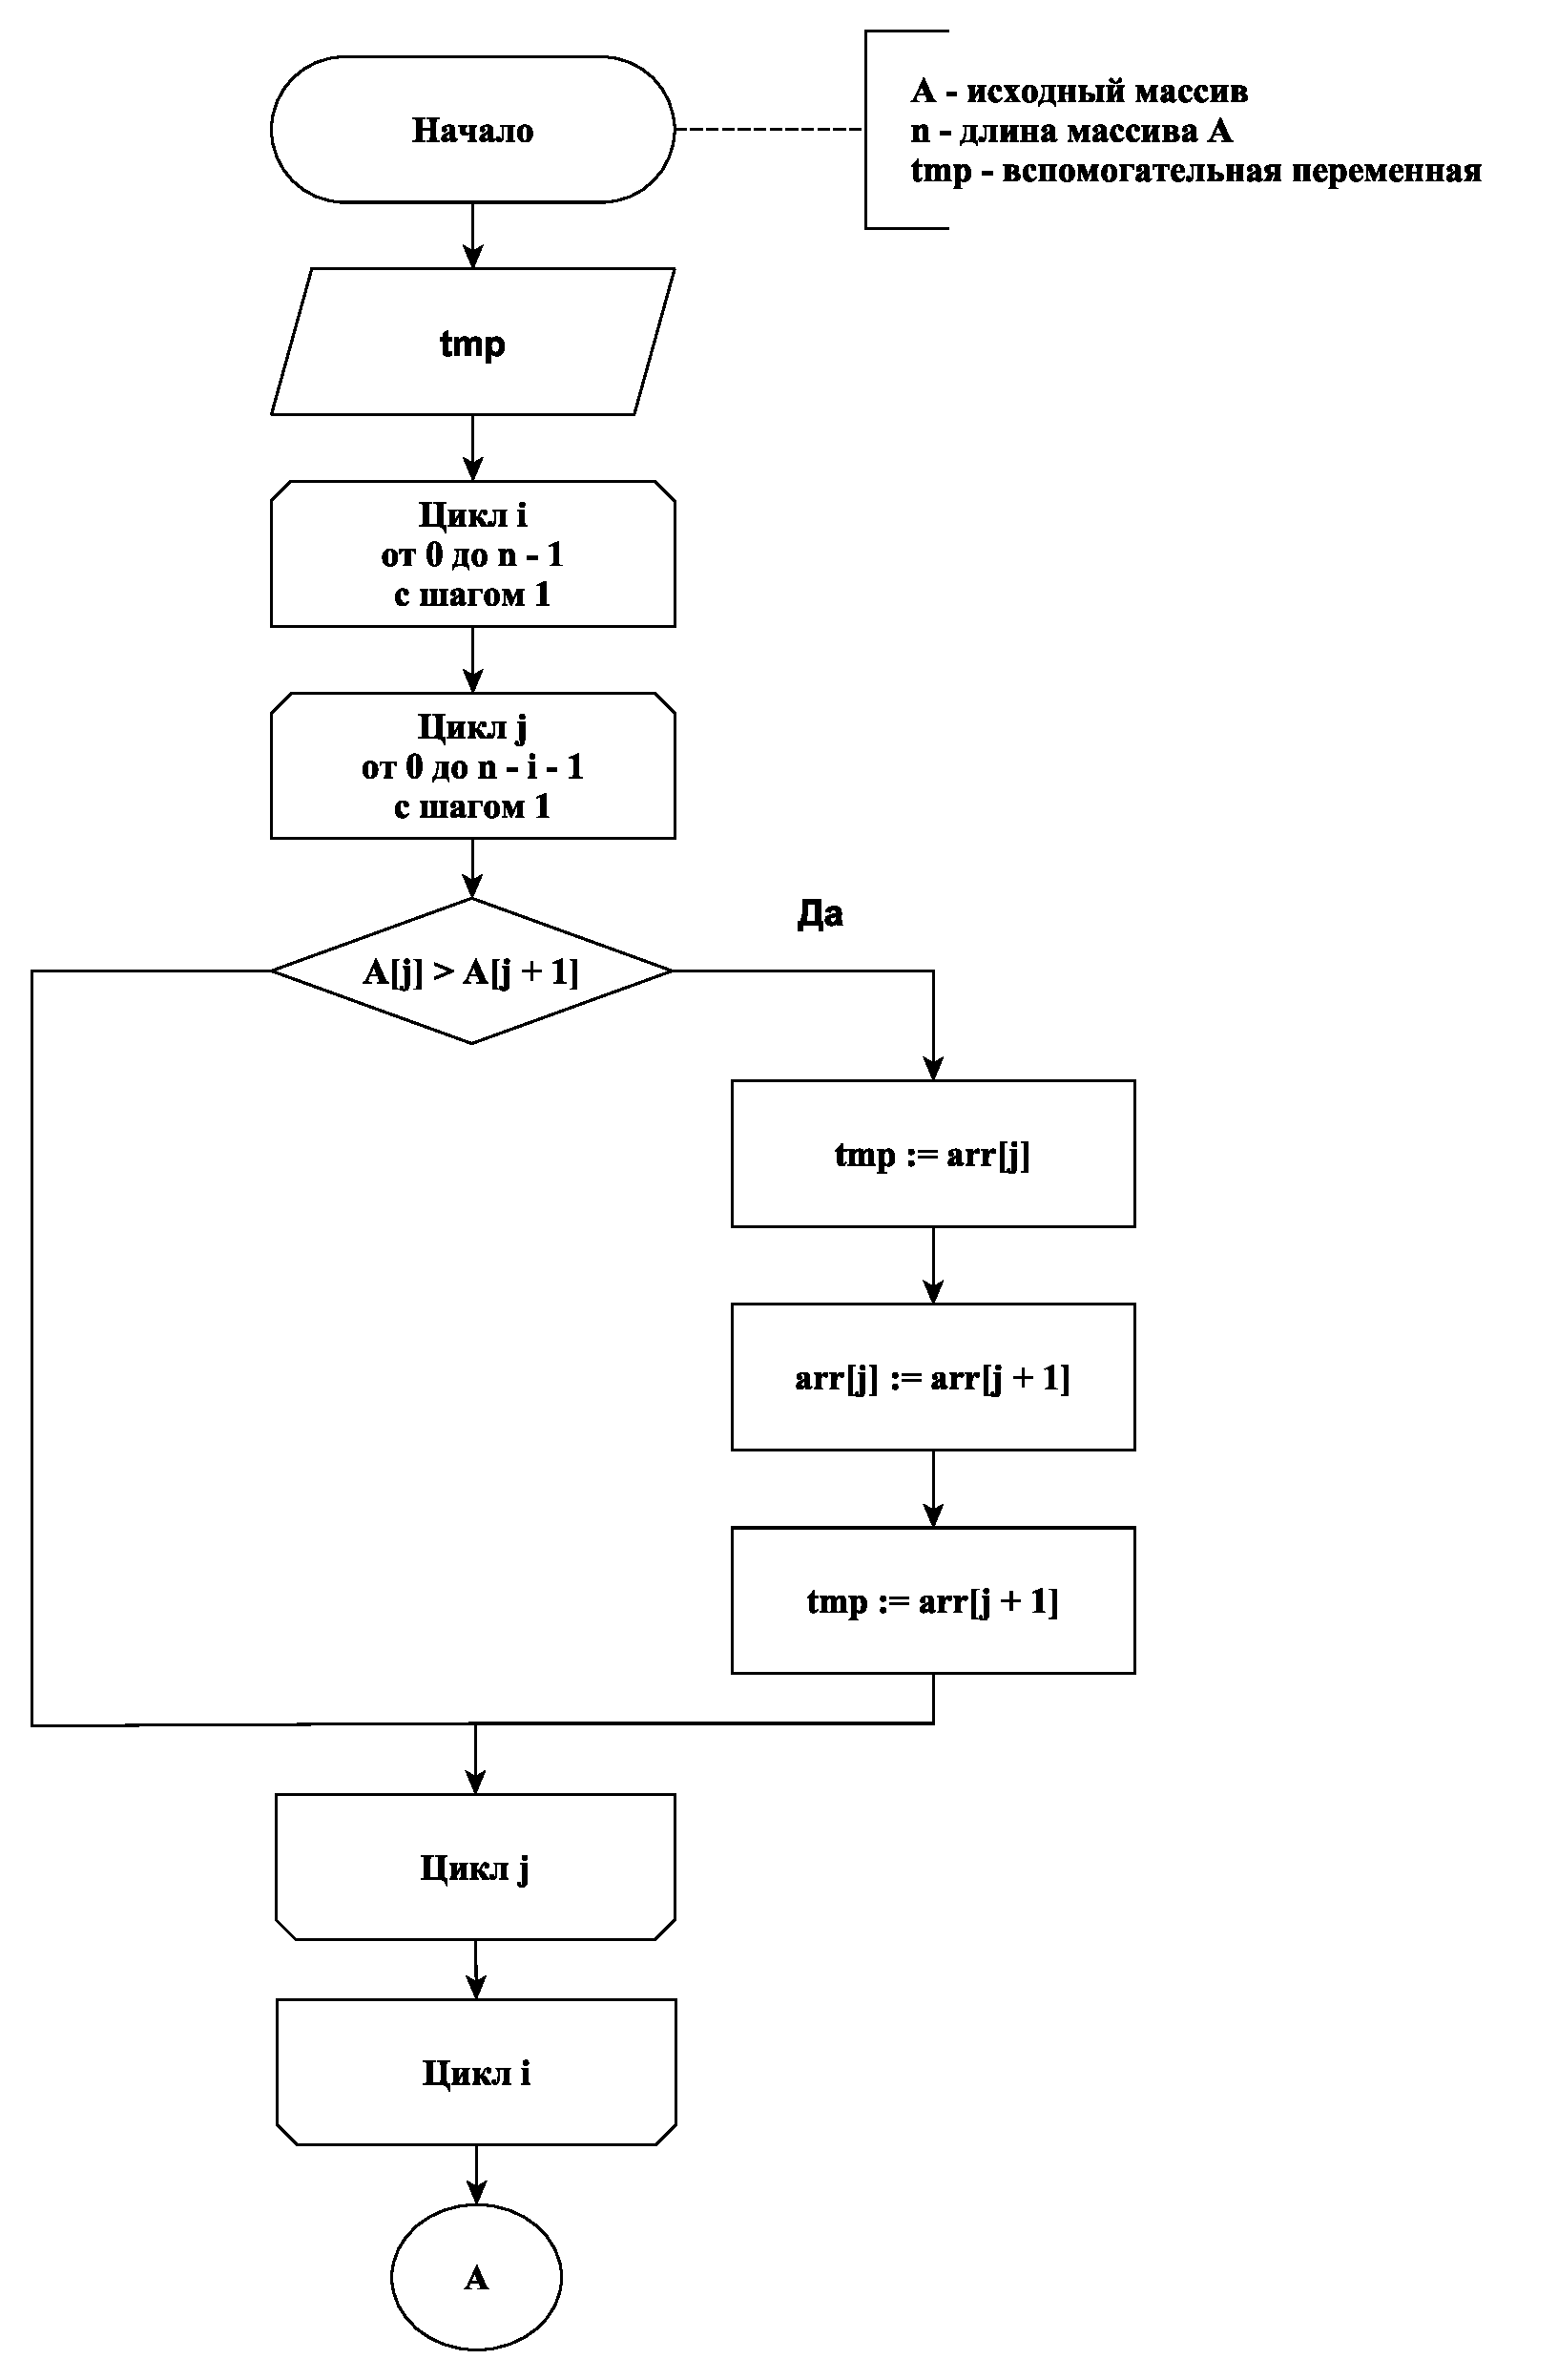
\includegraphics[scale = 0.45]{schema01.pdf}}
        		\caption{Схема алгоритма сортировки пузырьком}
        		\label{fig:schema_bubble_sort}
        	\end{center}
        \end{figure}
        
        
        \begin{figure}[h!]
        	\begin{center}
        		{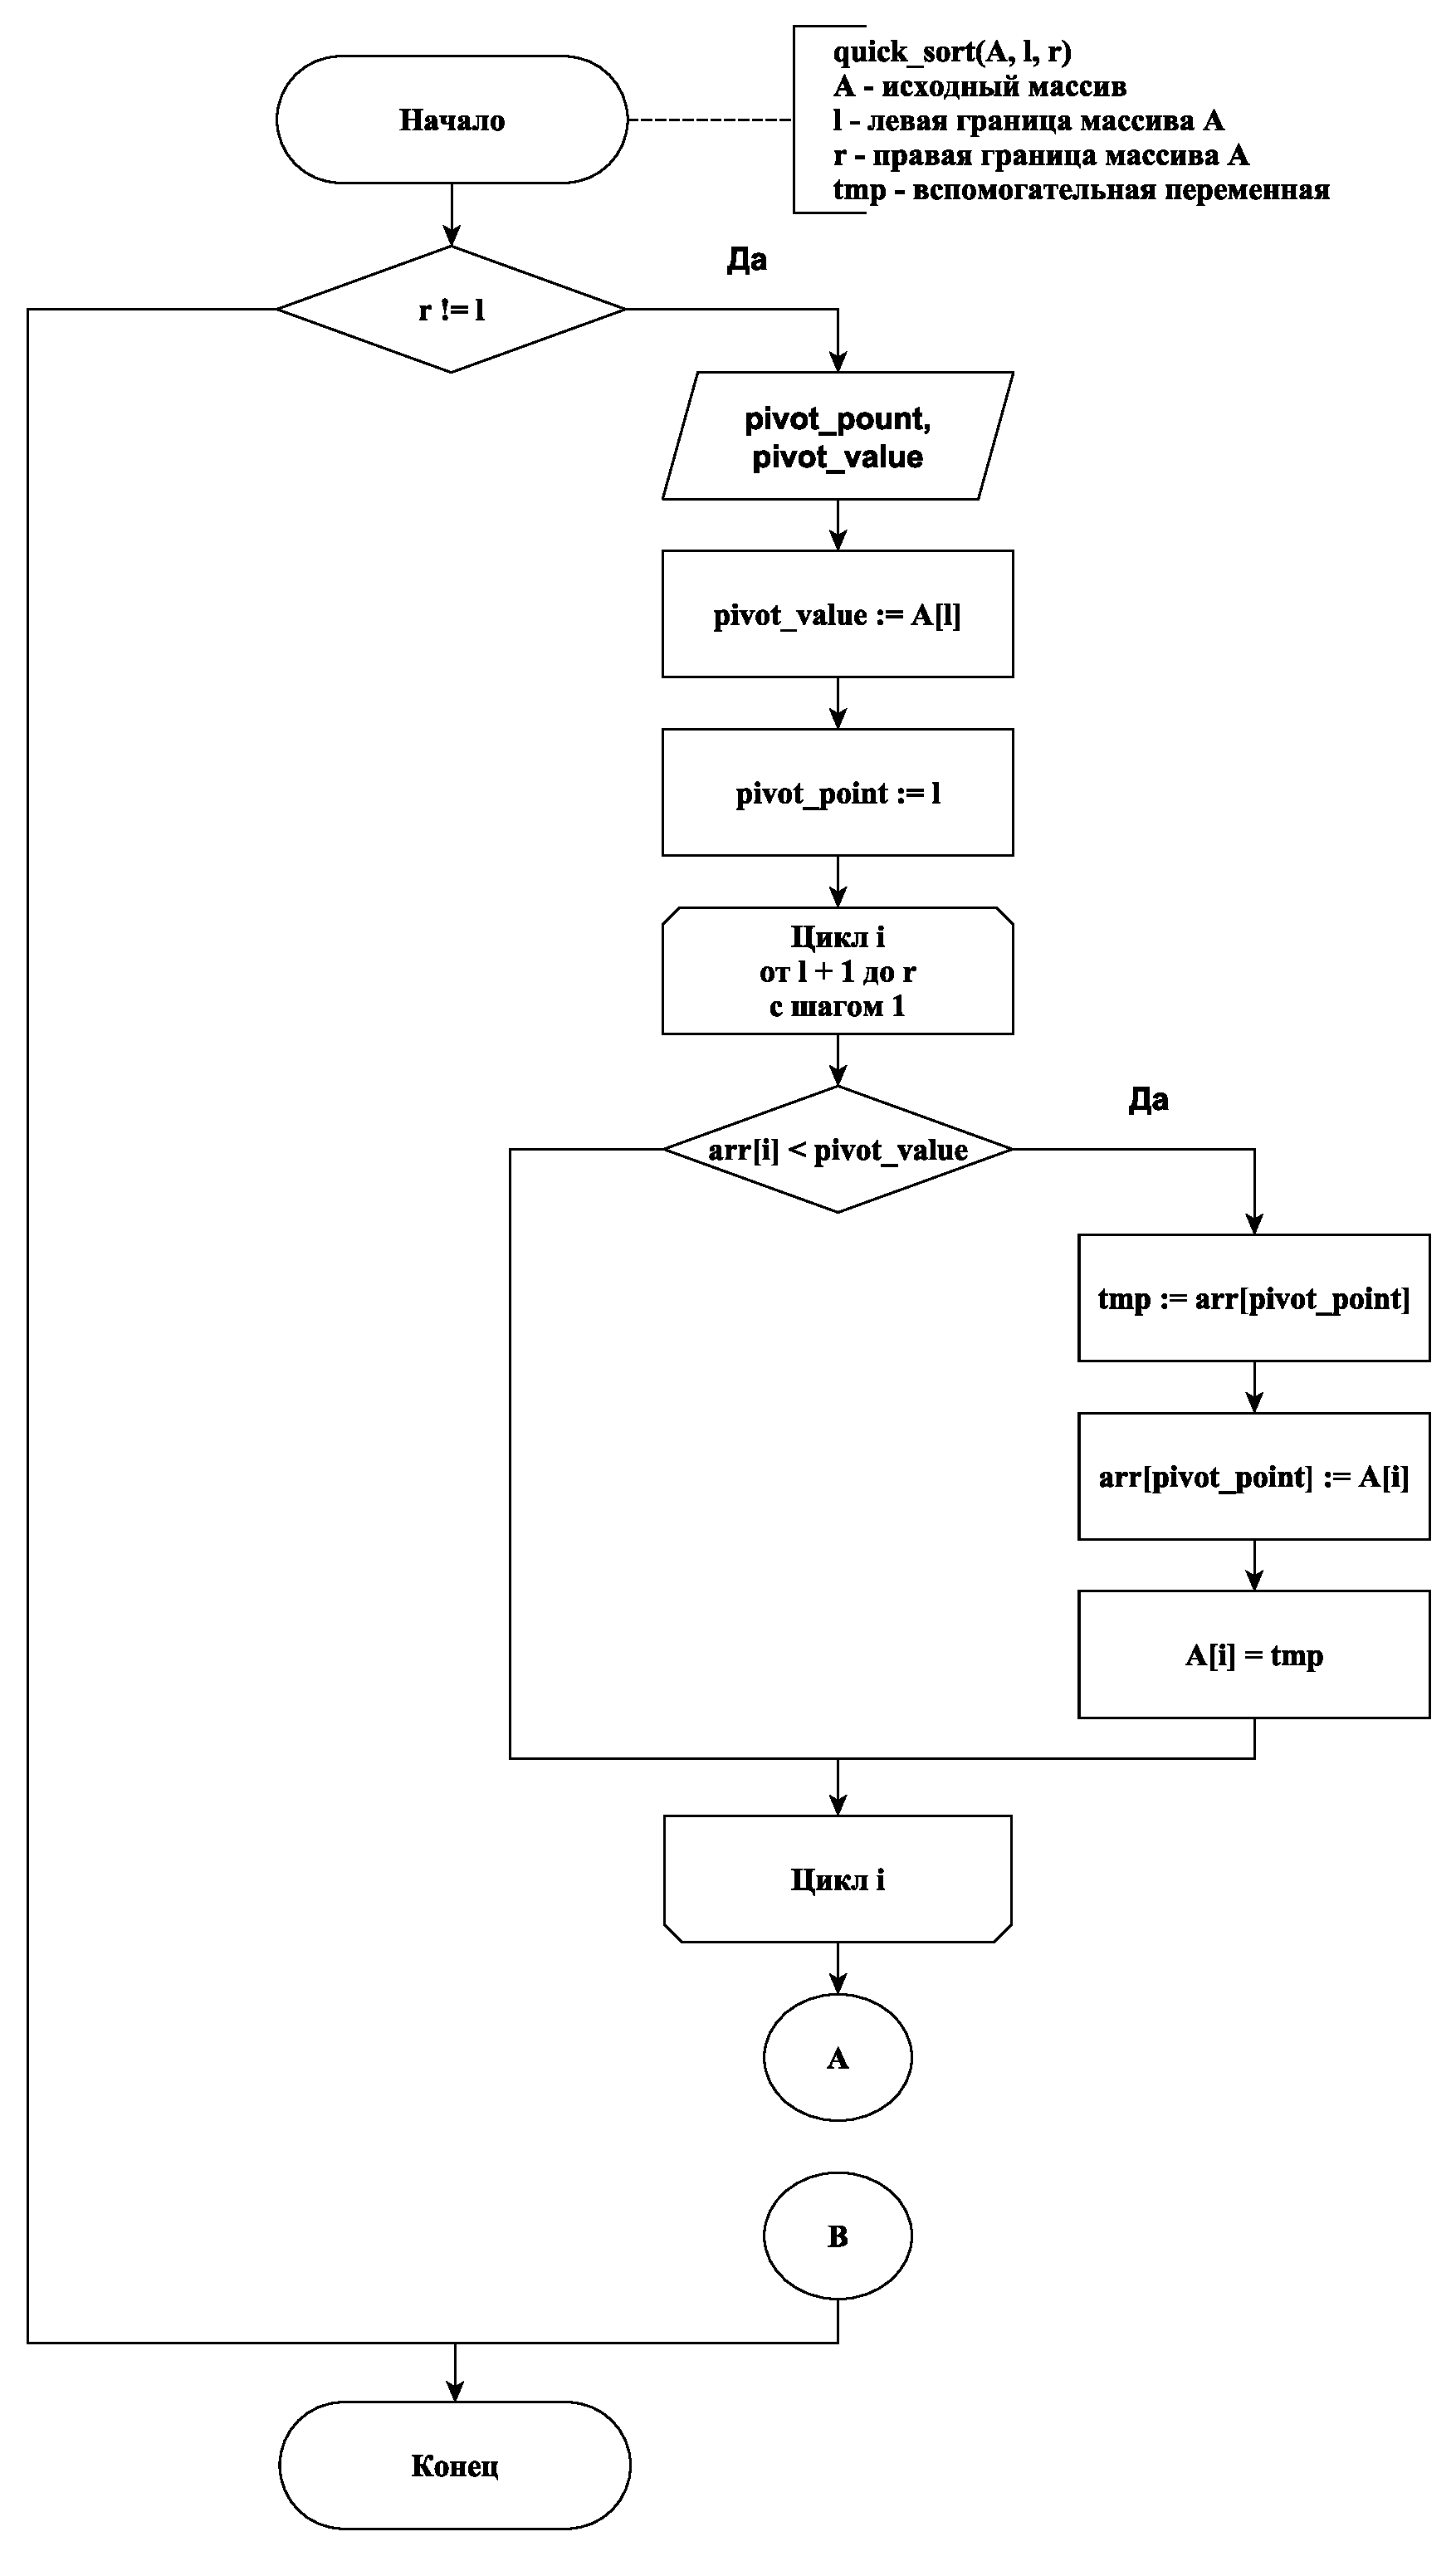
\includegraphics[scale = 0.47]{schema02.pdf}}
        		\caption{Схема алгоритма быстрой сортировки (часть 1)}
        		\label{fig:schema_quick_sort_1}
        	\end{center}
        \end{figure}
        
        \begin{figure}[h!]
        	\begin{center}
        		{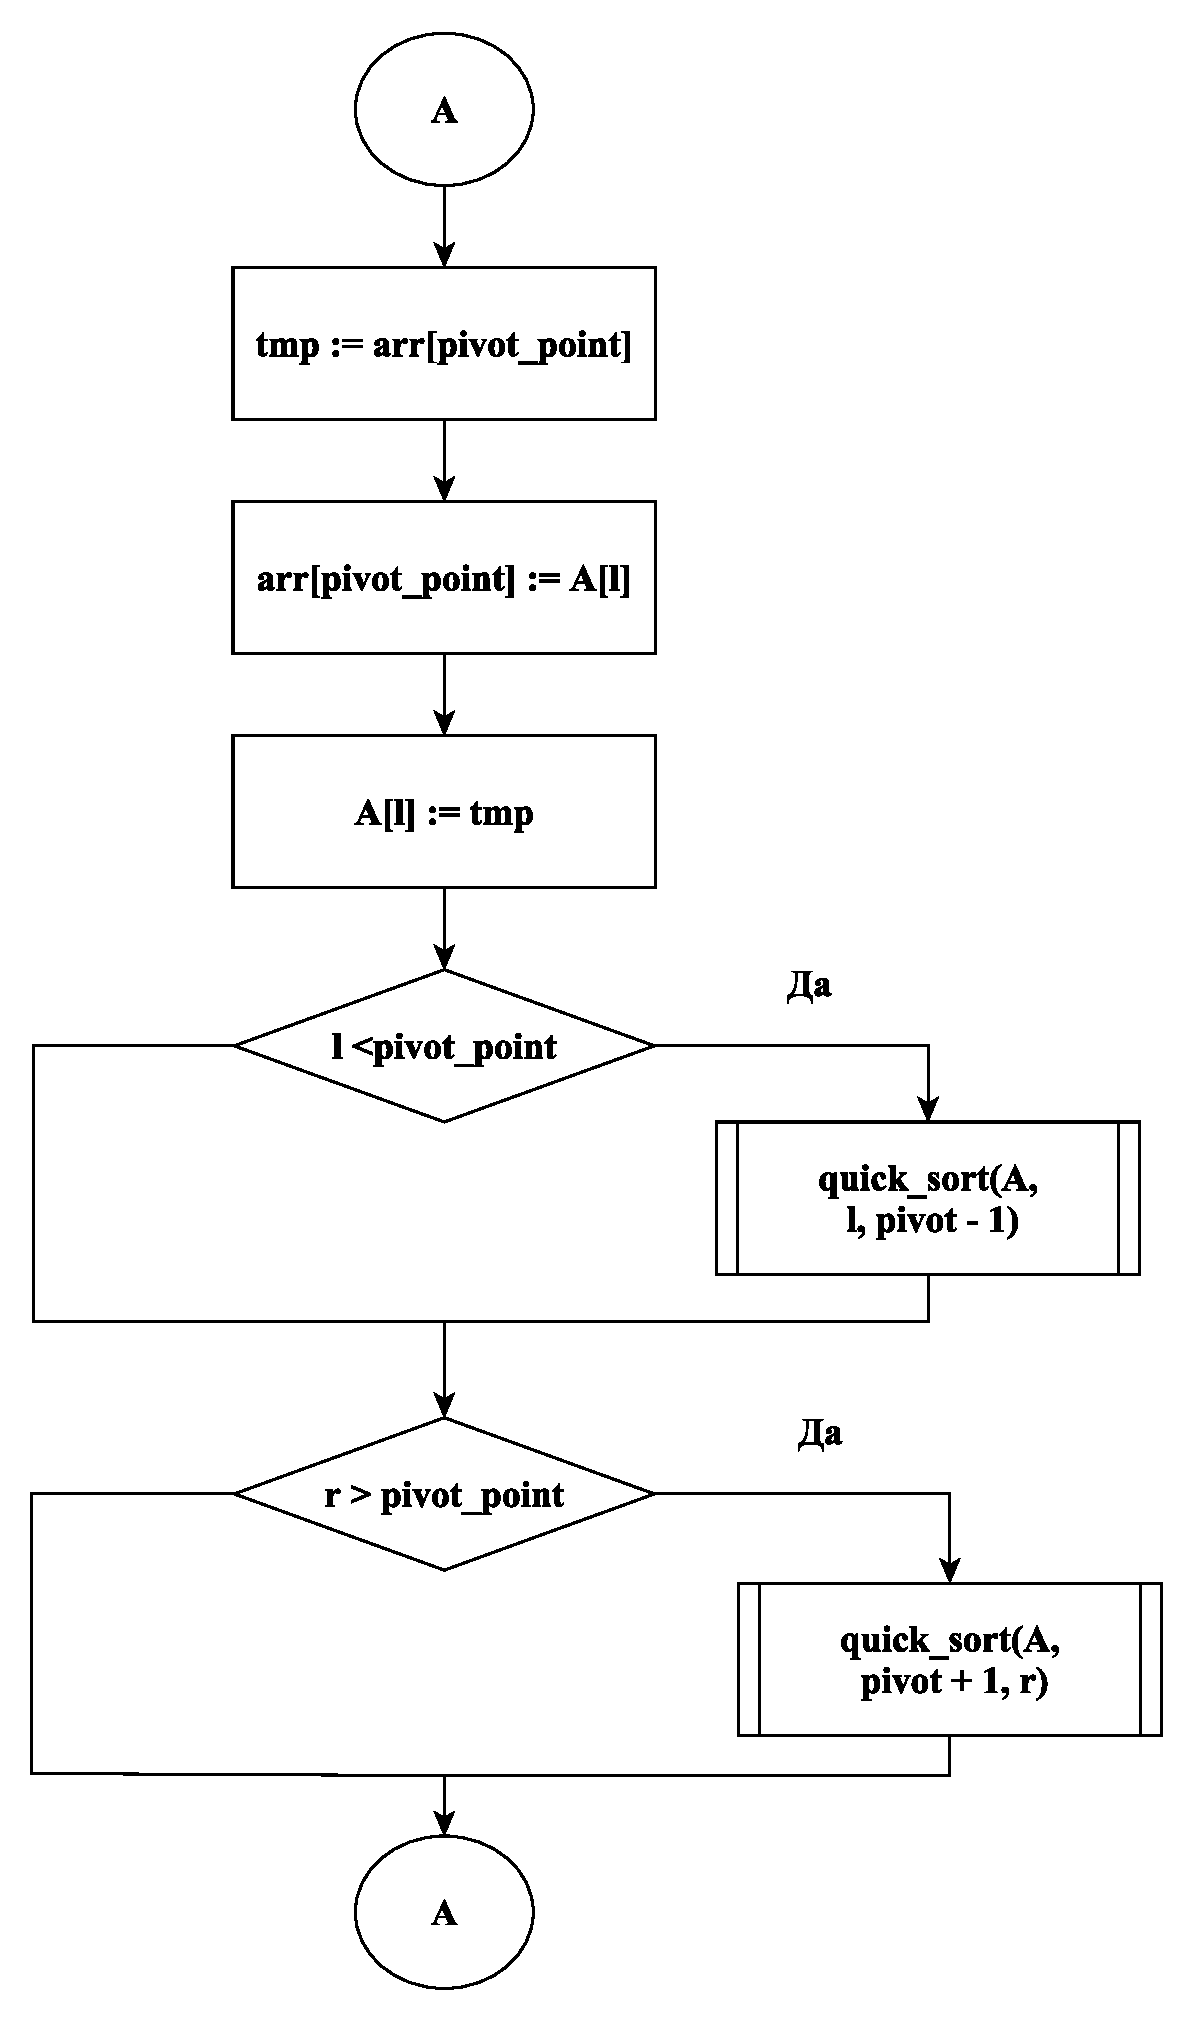
\includegraphics[scale = 0.55]{schema03.pdf}}
        		\caption{Схема алгоритма быстрой сортировки (часть 2)}
        		\label{fig:schema_quick_sort_2}
        	\end{center}
        \end{figure}
    
    
	    
	    \begin{figure}[h!]
	    	\begin{center}
	    		{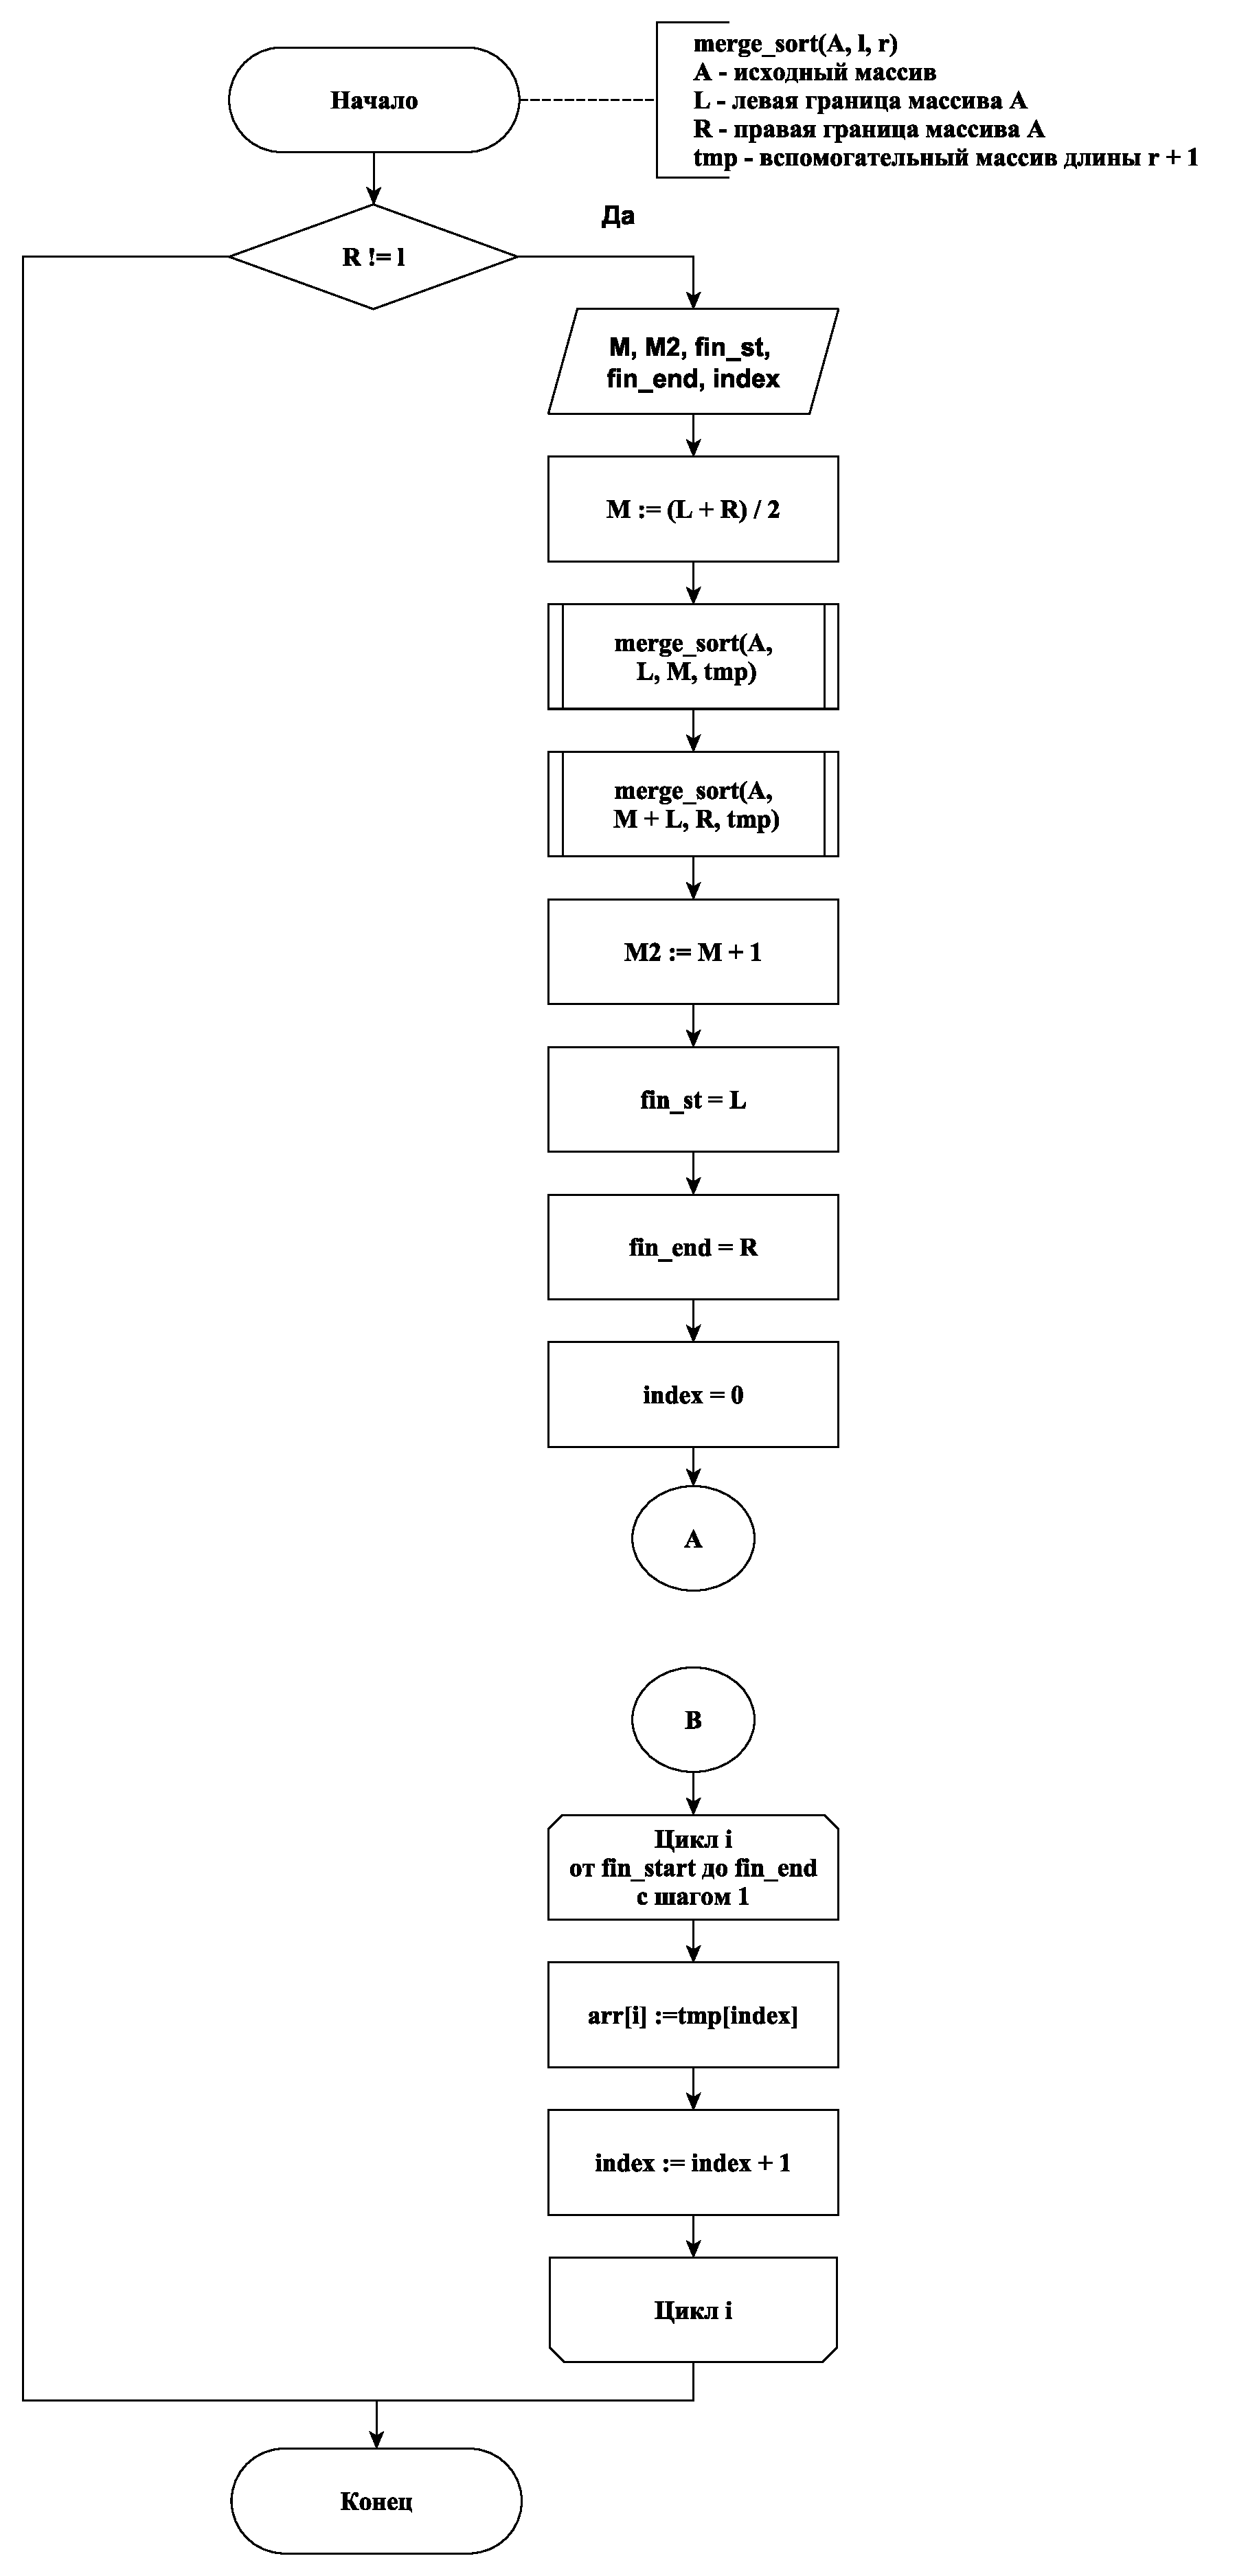
\includegraphics[scale = 0.38]{schema04.pdf}}
	    		\caption{Схема алгоритма сортировки слиянием (часть 1)}
	    		\label{fig:schema_merge_sort_1}
	    	\end{center}
	    \end{figure}
	    
	    \begin{figure}[h!]
	    	\begin{center}
	    		{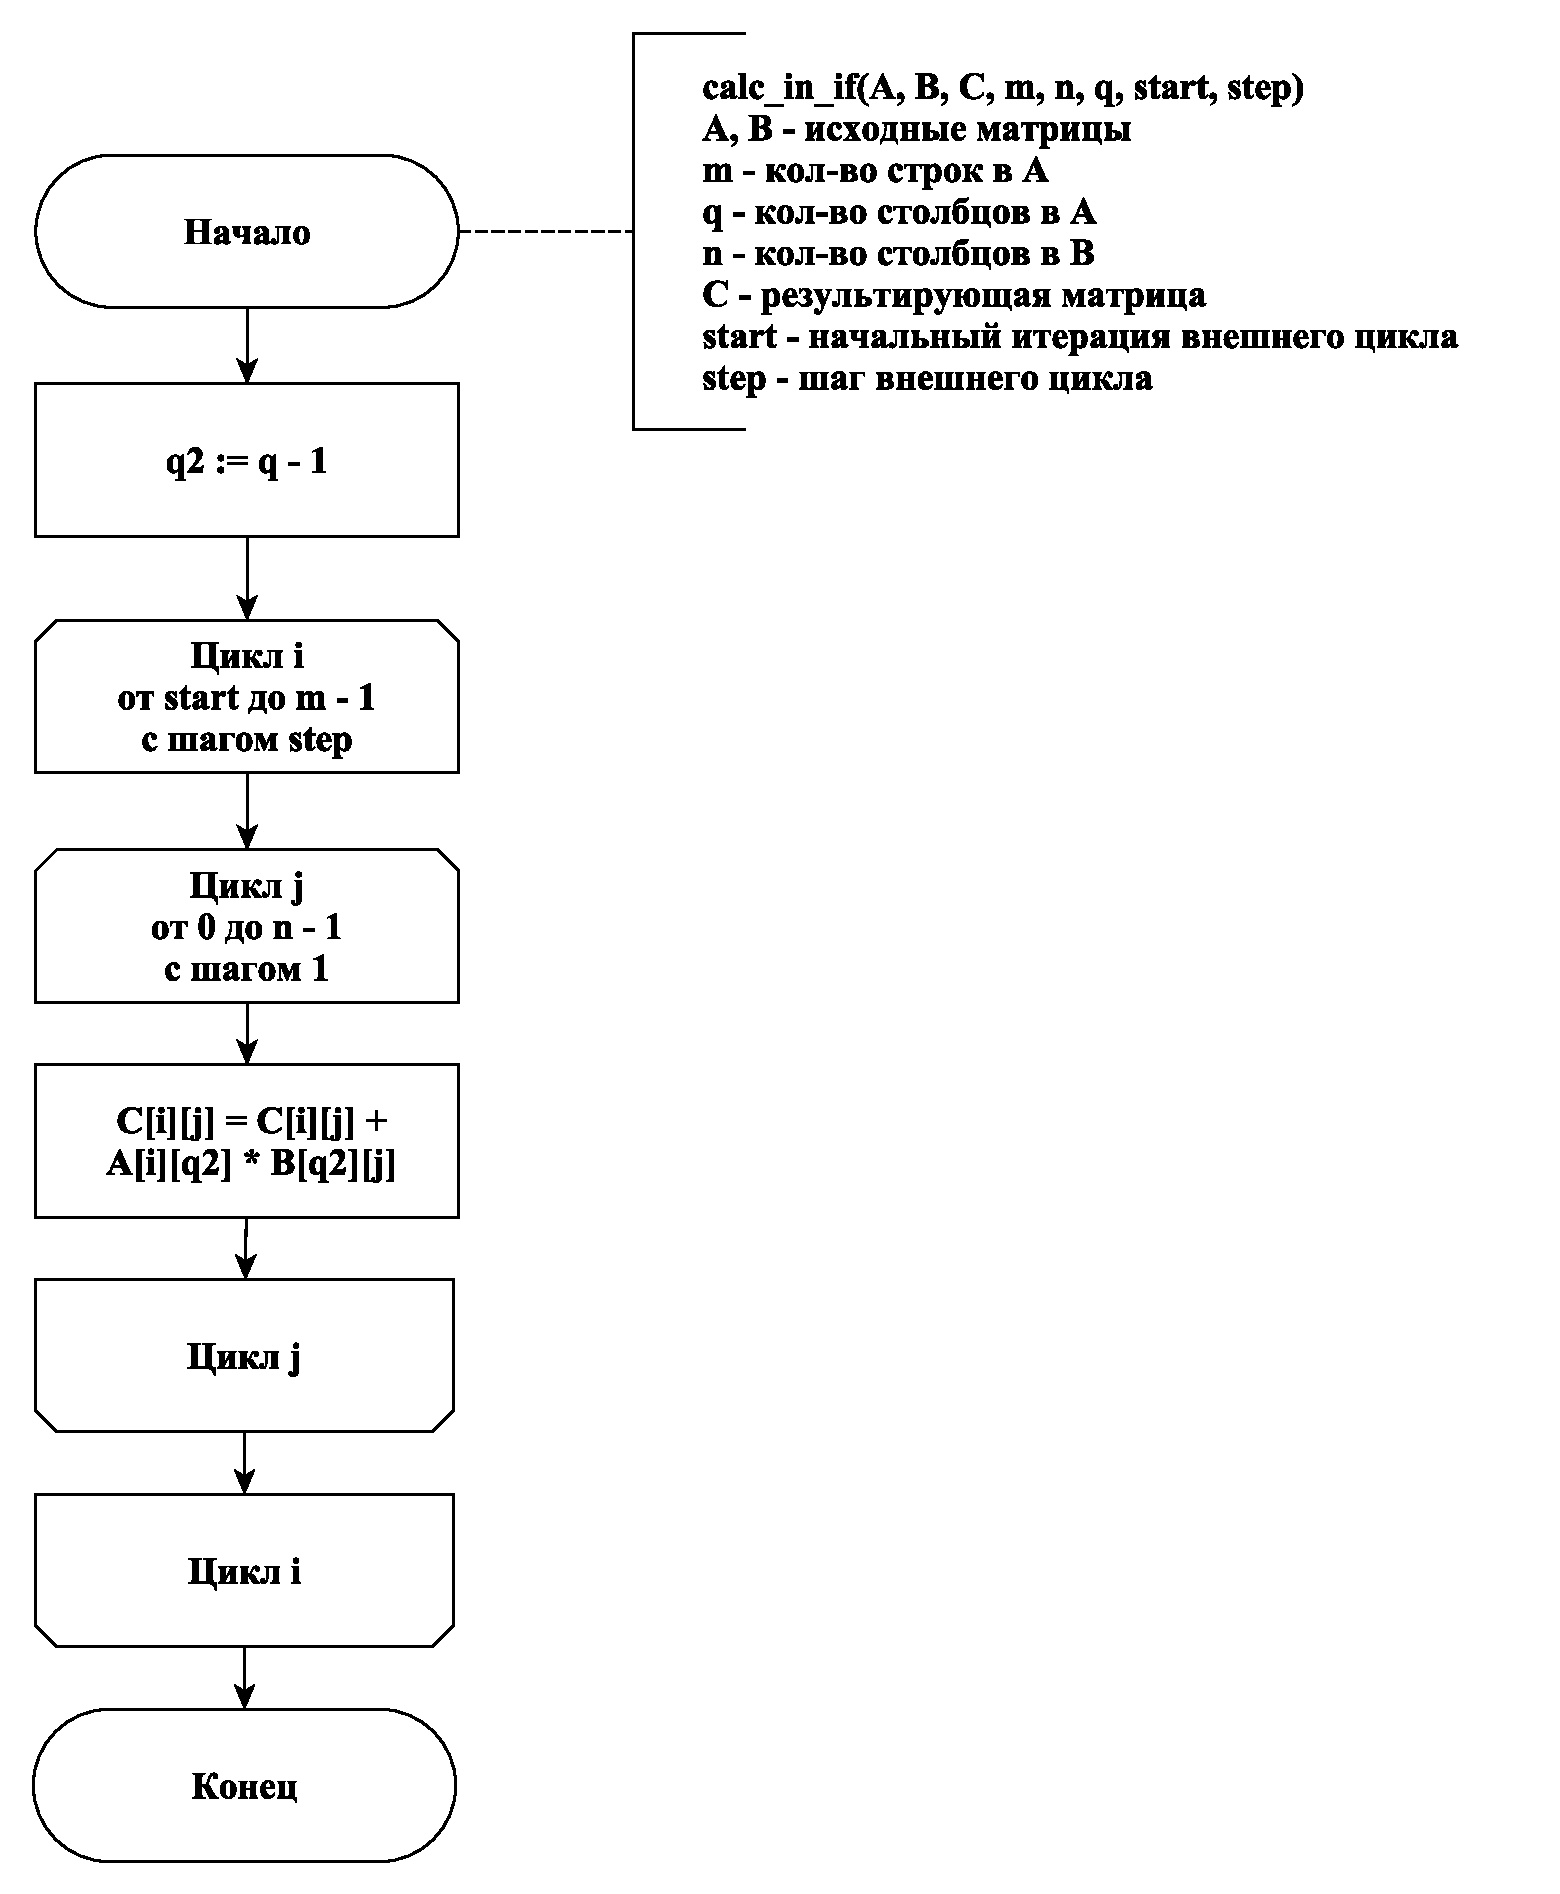
\includegraphics[scale = 0.48]{schema05.pdf}}
	    		\caption{Схема алгоритма сортировки слиянием (часть 2)}
	    		\label{fig:schema_merge_sort_2}
	    	\end{center}
	    \end{figure}
	\newpage
	\mbox{}
	\newpage

	\subsection{Сравнительный анализ алгоритмов}
	 \label{fig:an_alg}
		Трудоемкость алгоритмов измеряется в количестве необходимых операций.
		
		Введем модель вычислений:
		\begin{enumerate}
		\item[1)] Базовые операции стоимостью 1: +, -, /, *, =, ==, <=, >= !=, +=, -=, *=, /=, [\:].
		\item[2)] Стоимость цикла:
		\[
		f_{\text{цикла}} = f_{\text{иниц}} + f_{\text{сравн}} + N(f_{\text{тела}} + f_{\text{инкр}} + f_{\text{сравн}}) = 2 + N(f_{\text{тела}} + 2)
		\]
		\item[3)]  Стоимость условного перехода примем за 0, стоимость вычисления условия остается
		
		\end{enumerate}
		Найдем вычислительную сложность алгоритмов для массива длиной N элементов.
		\subsubsection{Сортировка пузырьком}
		В общем виде формула количества затрачиваемых операций выглядит так:
		\[
			f = \underbrace{2}_{=} + 2 + N\left(2 + 2 +\frac{N}{2}\left(2 + \underbrace{4}_{if} + 				\left [
		\begin{aligned}
		&0,  \text{если требуется обмен элементов} \\
		&\underbrace{4}_{[\:]} + \underbrace{3}_{=} + \underbrace{2}_{+}, \text{иначе}.
		\end{aligned}
		\right.\right)\right),		
		\]
		Лучшим случаем для алгоритма пузырька является уже упорядоченный массив, когда не будет происходить обмен элементов и сложность составит:
		\[
		f = 5 + N(4 +\frac{N}{2}\times(6 + 0)) = 3NN + 4N + 5.		
		\]
		Худшим, соответственно, будет случай когда массив отсортирован в обратном порядке, тогда на каждой итерации внутреннего цикла понадобится обмен и сложность будет:
		\[
		f = 5 + N(4 +\frac{N}{2}\times(6 + 9)) = \frac{15}{2}NN + 4N + 5.			
		\]
		
		Тогда для среднего случая сложность будет:
		\[
		f =  \frac{3  + \frac{15}{2}}{2}NN + 4N + 5	= \frac{21}{4}NN + 4N + 5.	
		\]
		
		Отсюда видно, что при любом случае сложность алгоритма $O(N^2)$
		\subsubsection{Сортировка слиянием}
		
		Оценим сначала трудоемкость слияния двух отсортированных массивов длиной $N_A$ и $N_B$. Лучшим случаем будет ситуация, когда все элементы одного больше (меньше) всех элементов другого. В таком случае, мы переносим в результирующий массив сначала все элементы одного массива, затем другого при минимальном количестве сравнений. Пусть Все элементы массива $N_A$ меньше всех элементов массива $N_B$, тогда:

		\[
			f(N_A, N_B) = \underbrace{4}_{=} + \underbrace{1}_{+} + 2 + N_A(2 + \underbrace{4}_{[\:]} + \underbrace{2}_{=} + \underbrace{1}_{+} + \underbrace{1}_{<}) + \underbrace{1}_{<} + 2 + \]
			\[   + N_B(3 + \underbrace{2}_{[\:]} + \underbrace{1}_{=})+ \underbrace{1}_{=} + 2 + (N_A + N_B)(3 + \underbrace{2}_{[\:]} + \underbrace{1}_{=})	=\]	
			\[   = 16N_A + 12N_B + 13. \]	
		
		
		Худшим случаем является случай, когда значения массив $N_A$ и $N_B$ идут <<через один>>, например 1-й элемент $N_A$ меньше 1-го элемента $N_B$, 1-й элемент $N_B$ меньше 2-го элемента $N_A$ и т. д. В таком случае сложность будет:
		
				\[
			f(N_A, N_B) = \underbrace{4}_{=} + \underbrace{1}_{+} + 2 + (N_A + (2 + \underbrace{4}_{[\:]} + \underbrace{2}_{=} + \underbrace{1}_{+} + \underbrace{1}_{<}) + \underbrace{1}_{<} + 2 \]
			\[   + (N_A + N_B)(3 + \underbrace{2}_{[\:]} + \underbrace{1}_{=})	=\]	
			\[   = 16N_A + 16N_B + 10. \]
			
			
		Теперь оценим саму сортировку. На каждой итерации происходит разбиение массива длины N на два длины $\frac{N}{2}$. Для их слияния понадобится в худшем случае $16N + 10$ операций и $14N + 10$ операций в худшем случае. Получаем рекуррентные соотношения на сложность в наихудшем (W) и наилучшем (В)
случаях:
\[
W(N) = 2W(16N) + 13,
\]
\[
W(0) = W(1) = 0;
\]
\[
B(N) = 2B(14N) + 10,
\]
\[
B(0) -5(1) = 0.
\]

Решив эти рекуррентные соотношения, получим значения близкие к приведенным в книге Дж. Макконнелла <<Анализ алгоритмов. Активный обучающий подход>> для худшего случая:
		\[
		f = N \log_2 N - N + 1.
		\]
		Для лучшего случая~\cite{makkonell}:
		\[
		f = \frac{N \log_2 N}{2}.
		\]
		
		Отбросив константное значение видим, что при любом случае алгоритм имеет асимптотику $O(N\log N)$
		\subsubsection{Быстрая сортировка}
			
		Худшим случаем для быстрой сортировки является отсортированный в каком-либо направлении массив, т. к. в этом случае в каждом рекурсивном вызове массив разбивается на два других, один из которых пуст, а другой целиком содержит укороченный на 1 элемент исходный массив. Таким образом сложность для худшего случая:
		\[
		f = \underbrace{2}_{=} + \underbrace{1}_{+} + \frac{N}{2}(\underbrace{2}_{>} + \underbrace{3}_{=} + \underbrace{1}_{==} + \underbrace{1}_{[\:]} + 3 + \]
		\[ + N(2 + \underbrace{1}_{=} + \underbrace{1}_{[\:]} + \underbrace{1}_{<}+ \underbrace{9}_{swap}) + \underbrace{9}_{swap}) =
		\]
		\[
		 = 7NN + 5N + 12
		\]
		
		В среднем случае, когда элементы массива достаточно перемешаны, скорость работы алгоритма определяется следующим рекуррентным соотношением ~\cite{makkonell}:
		\[
		A(N) = (N - 1) + \frac{1}{N} \left( 2\sum_{i=1}^{N - 1}A_i\right)  \text {для N > 2}
		\]
		\[
		A(1) = A(0) = 1
		\]
		
		Проанализировав их, получим:
		\[
		f \approx 1.4(N + 1) \log_2 N
		\]
		
		Таким образом, в худшем случае быстрая сортировка имеет сложность $O(N^2)$, а в среднем $N \log N$

	    
	\subsection*{Вывод}
		\addcontentsline{toc}{subsection}{Вывод}
		В данном разделе были представлены схемы сортировки пузырьком, сортировки слиянием и быстрой сортировки.
			Был произведен аналитический анализ трудоемкости сортировок, в ходе которого выяснилось, что самой эффективной является сортировка слиянием, имеюшая сложность $O(N\log_2 N)$ на любом массиве. Быстрая сортировка в среднем случае также имеет сложность $O(N\log_2 N)$, но в худшем случае (когда массив изначально отсортирован в прямом или обратном порядке) имеет сложность $O(N^2)$. Сортировка пузырьком является самой медленной - при любых исходных данных она имеет сложность $O(N^2)$. 


  
\pagebreak
\newpage         

\section{Технологический раздел}

	В данном разделе будут описаны требования к программному обеспечению и средства реализации, приведен листинг программы и выполнен сравнительный анализ трудоемкости алгоритмов.
	\subsection{Требования к программному обеспечению}
	Входные данные: 
	 \begin{enumerate} 
	 \item[1)] целое положительное число - размерность массива: N;
	 \item[2)] массив, заполненный вещественными числами.
	 \end{enumerate}
	
	Выходные данные: исходный массив, отсортированный по возрастанию.
	
	На рис. \ref{fig:idef0} приведена функциональная схема сортировки массива.
        
        \begin{figure}[h!]
        	\begin{center}
        		{\includegraphics[width = \textwidth]{idef0.png}}
        		\caption{Функциональная схема сортировки массива}
        		\label{fig:idef0}
        	\end{center}
        \end{figure}
        
	
	\subsection{Средства реализации}
	Программа написана на языке С++, т. к. этот язык предоставляет программисту широкие возможности реализации самых разнообразных алгоритмов, обладает высокой эффективностью и значительным набором стандартных классов и процедур. В качестве среды разработки использовался  фреймворк QT 5.13.1.
	
	Для обработки массивов был использован стандартный контейнерный класс std::vector.
	
	Для замера времени выполнения программы использовалась библиотека chrono.
	

    
    \subsection{Листинг программы}
	В листингах \ref{code_std},  \ref{code_vin} и \ref{code_vin_opt} представлены функции сортировки пузырьком, сортировки слиянием и быстрой сортировки.
	
	\begin{center}
	\begin{lstlisting}[label=code_std, caption={Сортировка пузырьком}]
void bubble_sort(Vector &arr) {
    size_t n = arr.size();
    double tmp = 0;
    for (size_t i = 0; i < n - 1; i++) {
        for (size_t j = 0; j < n - i - 1; j++) {
            if (arr[j] > arr[j + 1]) {
                std::swap(arr[j], arr[j + 1]);
            }
        }
    }
}

    \end{lstlisting}
    \end{center}  

     
	\begin{lstlisting}[label=code_vin, caption={Быстрая сортировка}]
void quick_sort(Vector &arr, size_t l, size_t r) {
    if (r == l) return;
    size_t pivot = pivot_arr(arr, l, r);
    if (l < pivot) {
        quick_sort(arr, l, pivot - 1);
    }
    if (r > pivot) {
        quick_sort(arr, pivot + 1, r);
    }
}

size_t pivot_arr(Vector &arr, size_t l, size_t r) {

    double pivot_value = arr[l];
    size_t pivot_point = l;
    for (size_t i = l + 1; i <= r; i++) {
        if (arr[i] < pivot_value) {
            pivot_point++;
            std::swap(arr[pivot_point], arr[i]);
        }
    }
    std::swap(arr[l], arr[pivot_point]);
    return pivot_point;

}
\end{lstlisting}


	\begin{lstlisting}[label=code_vin_opt, caption={Сортировка слиянием}]
void merge_sort(Vector &arr, size_t l, size_t r, Vector &tmp) {
    if (l == r) return;
    size_t m = (l + r) / 2;
    merge_sort(arr, l, m, tmp);
    merge_sort(arr, m + 1, r, tmp);
    merge(arr, l, m, r, tmp);
}

void merge(Vector &arr, size_t st1, size_t end1, size_t end2, Vector &tmp) {
    size_t st2 = end1 + 1;
    size_t fin_st = st1;
    size_t fin_end = end2;
    size_t index = 0;
    while (st1 <= end1 && st2 <= end2) {
        if (arr[st1] < arr[st2]) {
            tmp[index] = arr[st1];
            st1++;
        }
        else {
            tmp[index] = arr[st2];
            st2++;
        }
        index++;
    }

    if (st1 <= end1) {
        for (size_t i = st1; i <= end1; i++, index++) {
            tmp[index] = arr[i];
        }
    }
    else {
        for (size_t i = st2; i <= end2; i++, index++) {
            tmp[index] = arr[i];
        }
    }

    index = 0;
    for (size_t i = fin_st; i <= fin_end; i++, index++) {
        arr[i] = tmp[index];
    }


}

    \end{lstlisting}  
    
%    
    \subsection{Тестовые данные}
    \label{fig:test_data}

    Программа должна корректно сортировать массив при следующих входных данных:
     \begin{table} [h!]
    \begin{center}
    \caption{Тестовые данные} 
    \begin{tabular}{|c|p{7cm}|p{7cm}|}
    \hline
№ & Исходный массив & Отсортированный массив \\
    	\hline
    	1 & \{1\} & \{1\}  \\
    	\hline
    	2 & \{2, 1\} & \{1, 2\}  \\
    	\hline
    	3 & \{1, 2, 3, 4, 5\} & \{1, 2, 3, 4, 5\} \\
    	\hline
    	4 & \{5, 4, 3, 2, 1\} & \{1, 2, 3, 4, 5\}   \\
    	\hline
    	5 & \{2, 2, 2\} & \{2, 2, 2\}   \\
    	\hline
    	6 & \{5, 2, 3, 4, 1\} & \{1, 2, 3, 4, 5\}   \\
    	\hline
    	7 & \{-5, -4, -3, -2, -1\} & \{-5, -4, -3, -2, -1\}  \\
    	\hline
    	8 & \{-5, 4, -3, 2, -1, 0\} & \{-5, -3, -1, 0, 2, 4\}   \\
    	\hline
    	9 & \{1, 1, 3, 6, 1, 5, 9, 3\} & \{1, 1, 1, 3, 3, 5, 6, 9\}  \\
    	\hline
    	10 & \{3.98, 0, 4.1, -2.34, 10.876, 3.99, -8\} & \{-8, -2.34, 0, 3.98, 3.99, 4.1, 10.876\}  \\
    	\hline
    	11 & \{1000, -2000, 3000, 0, 5000, -9000, -5000\} & \{-9000, -5000, -2000, 0, 1000, 3000, 5000\}  \\
    	\hline

    	
    \end{tabular} \\
	\label{table:test_data_table}
    \end{center}
    \end{table}
    \newpage    	
    Все тесты успешно пройдены.
		
		
	
	
	\subsection*{Вывод}
		\addcontentsline{toc}{subsection}{Вывод}
	
	В данном разделе были рассмотрены требования к программному обеспечению, в качестве средств реализации выбраны язык С++ и фреймворк QT версии 5.13.1, приведён листинг программы и тестовые данные. Все тесты успешно прошли тестирование, результаты совпали с ожидаемыми.
	

\pagebreak

\section{Исследовательский раздел}

    
    \subsection{Примеры работы}
        
        На рис. \ref{fig:image_test_1}, \ref{fig:image_test_2}, \ref{fig:image_test_3}, \ref{fig:image_test_4} и \ref{fig:image_test_5} приведены примеры работы программы для различных входных данных. 
        
        	\begin{figure}[h!]
                \center{\includegraphics[scale = 0.7]{test03.png}}
                \caption{Пример работы программы для некорректного ввода}
                \label{fig:image_test_1}
            \end{figure}
            
            
            \begin{figure}[h!]
                \center{\includegraphics[scale = 0.7]{test02.png}}
                \caption{Пример работы программы для отсортированного массива }
                \label{fig:image_test_2}
            \end{figure}        
        
            \begin{figure}[h!]
                \center{\includegraphics[scale = 0.7]{test04.png}}
                \caption{Пример работы программы для отсортированного в обратном порядке массива}
                \label{fig:image_test_3}
            \end{figure}
            
               \begin{figure}[h!]
                \center{\includegraphics[scale = 0.7]{test04.png}}
                \caption{Пример работы программы для неупорядоченного массива}
                \label{fig:image_test_4}
            \end{figure}
            
            \begin{figure}[h!]
                \center{\includegraphics[scale = 0.7]{test05.png}}
                \caption{Пример работы программы для массива с большими значениями}
                \label{fig:image_test_5}
            \end{figure}

    \subsection{Постановка эксперимента}
    
    Необходимо выполнить следующие замеры времени:
    \begin{enumerate} 
        \item Сравнить время сортировок алгоритмов на массивах с произвольно сгенерированными числами.
        \item Провести аналогичное сравнение на массивах, с самыми подходящими данными для конкретных алгоритмов (лучший случай). Для сортировки пузырьком это уже отсортированный массив, для быстрой сортировки - произвольно сгенерированный, для сортировке слиянием принципиальной разницы нет.
        \item Провести аналогичное сравнение на массивах, с самыми неподходящими данными для конкретных алгоритмов (худший случай). Для сортировки пузырьком это  массив, отсортированный в обратном порядке, для быстрой сортировки - отсортированный в любом направлении массив, для сортировке слиянием принципиальной разницы нет.
        
    \end{enumerate} 
    
    Все замеры произвести на массивах длиной от 100 до 1000 элементов с шагом 100, каждый замер выполняется 10000 раз.
    
    
    \subsection{Сравнительный анализ на материале экспериментальных данных}
        На рис. \ref{fig:gtaf_1} приводятся графики времени сортировки алгоритмов на массивах с произвольно сгенерированными числами.
        
        \begin{figure}[h!]
            \center{\includegraphics[width = \textwidth]{graf02.png}}
            \caption{Время выполнения алгоритмов на массивах с произвольно сгенерированными числами}
            \label{fig:gtaf_1}
        \end{figure}
        
        Как видно, сортировка пузырьком существенно проигрывает быстрой сортировке и сортировке слиянием. Графики соответствуют посчитанным в разделе \ref{fig:an_alg} асимптотикам для случайного массива:  $O(N^2)$ для пузырьковой сортировки и $O(N \log N)$ для быстрой сортировки и сортировки слиянием.
        
                На рис. \ref{fig:graf_2} приводятся графики времени сортировки алгоритмов при лучшем случаи.
         
        \begin{figure}[h!]
            \center{\includegraphics[width = \textwidth]{graf03.png}}
            \caption{Время выполнения алгоритмов при худшем случае}
            \label{fig:graf_2}
        \end{figure}
        
        Как видно, пузырек стал выполняться быстрее (1.5 мс на 1000 элементов, по сравнению с прежними 5-ю мс), характер зависимости при этом остался таким же как у замеров с произвольно заполненными массивами. Быстрая сортировка и сортировка слиянием сохранили свою асимптотику в $O(N \log N)$. 
        
         На рис. \ref{fig:graf_3} приводятся графики времени сортировки алгоритмов при худшем случае.
         
        \begin{figure}[h!]
            \center{\includegraphics[width = \textwidth]{graf01.png}}
            \caption{Время выполнения алгоритмов при лучшем случае}
            \label{fig:graf_3}
        \end{figure}
        
		Видно, что в данном случае быстрая сортировка существенно замедлилась, что соответствует ее теоретической оценке для худшего случая в $O(N^2)$. Пузырек   также упал в производительности по сравнению с замерами для среднего случая (7 секунд для массива в 1000 элементов, по сравнению с 5 секундами для замера с произвольными числами). Сортировка слиянием по-прежнему остается самой производительной.
		
	
        
       \subsection*{Вывод}
		\addcontentsline{toc}{subsection}{Вывод}
       В результате тестирования программой были успешно пройдены все заявленные тесты. Эксперименты замера времени показали, что самой эффективной является сортировка слиянием, которая вне зависимости от входных данных имеет сложность $O(N \log N)$. Однако ее недостатком является необходимость выделять память под вспомогательный массив. Быстрая сортировка в среднем случае также показывает сложность $O(N \log N)$, но в худшем случае (например, при отсортированном массиве) опускается до $O(N^2)$. Пузырек оказался самым неэффективным - его сложность в любом случае $O(N^2)$.
        
    

\pagebreak
\section*{Заключение}
\addcontentsline{toc}{section}{Заключение}
	В ходе работы было выполнено следующее:
	\begin{enumerate}
	\item[1)] изучены алгоритмы сортировок;
	\item[2)] применены методы динамического программирования для  
	реализации указанных алгоритмов;
	\item[3)] получены практические навыки реализации указанных алгоритмов: сортировки пузырьком, сортировки слиянием и быстрой сортировки;
	\item[5)] проведен сравнительный анализ алгоритмов по затрачиваемым ресурсам (времени);
	\item[4)] выполнено экспериментальное подтверждение различий во временнóй эффективности алгоритмов при помощи разработанного программного обеспечения на материале замеров процессорного времени на варьирующихся размерностях матриц;
	\item[5)] описаны и обоснованы полученные результаты в отчете о выполненной лабораторной работе, выполненного как расчётно-пояснительная записка к работе. 
	\end{enumerate}
	
	
	Аналитический анализ трудоемкости алгоритмов показал, что что самой эффективной является сортировка слиянием, имеюшая сложность $O(N\log N)$ на любом массиве. Быстрая сортировка в среднем случае также имеет сложность $O(N\log N)$, но в худшем случае (когда массив изначально отсортирован в прямом или обратном порядке) имеет сложность $O(N^2)$. Сортировка пузырьком является самой медленной - при любых исходных данных она имеет сложность $O(N^2)$.
	
	Экспериментальный анализ эффективности алгоритмов подтвердил теоретическую оценку. Пузырек был стабильно медленным на любых данных(в 100-150 раз медленнее других массивов на массиве длиной 1000 элементов в среднем и лучшем случаях). Слияние давало стабильный выигрыш на любых массивах). Быстрая сортировка в лучшем и среднем случаях была эффективна как и сортировка слиянием, а в худшем случае   шла наравне с пузырьком.
	


\pagebreak
\addcontentsline{toc}{section}{Список литературы}
\begin{thebibliography}{4}
\bibitem{makkonell}
Дж. Макконнелл. Анализ алгоритмов. Активный обучающий подход.-
М.:Техносфера, 2009.
\bibitem{habr}
Описание алгоритмов сортировки и сравнение их производительности [Электронный ресурс]. – Режим доступа: https://habr.com/ru/post/335920/, свободный – (22.10.2019)
\bibitem{bib}
Что такое сортировка? [Электронный ресурс]. – Режим доступа: https://dic.academic.ru/dic.nsf, свободный – (21.10.2019)
\bibitem{bubble}
Пузырьковая сортировка (Bubble-sort) [Электронный ресурс]. – Режим доступа: https://forkettle.ru/vidioteka/programmirovanie-i-set/108-algoritmy-i-struktury-dannykh/sortirovka-i-poisk-dlya-chajnikov/1004-puzyrkovaya-sortirovka, свободный – (21.10.2019)

\end{thebibliography}




\end{document} % Конец текста.
